\documentclass[10pt]{standalone}
\usepackage{amsmath}
\usepackage{pgf,tikz}
\usetikzlibrary{calc}
\usepackage{mathrsfs}
\usetikzlibrary{arrows}
\pagestyle{empty}
\begin{document}
	

	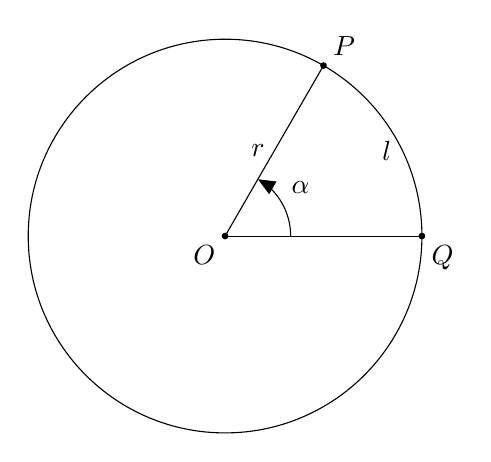
\begin{tikzpicture}[>=triangle  45]
	\tikzset{samples=600}
	\pgfmathsetmacro{\raggio}{2.5};
	\pgfmathsetmacro{\angolo}{60};
	\pgfmathsetmacro{\y}{3};
	\coordinate [label=below left:$O$] (oo)  at (0,0);
	\draw (oo) circle (\raggio) ;
	\filldraw[black] (oo) circle(1pt);
	\coordinate [label=above right:$P$] (P) at  ({\raggio*cos(\angolo)},{\raggio*sin(\angolo )});
	\coordinate[label=below right:$Q$] (Q) at (\raggio,0);
	\coordinate[label=right:$l$] (M)at ($(P)!0.5!(Q)$);
	\draw[->] (\raggio/\y,0 ) arc (0:\angolo:\raggio/\y);
	\draw (\angolo/2:\raggio/\y) node[ above right]  {$\alpha$};
	\filldraw[black] (Q) circle(1pt);
	\filldraw[black] (P) circle(1pt);
	\draw (oo)-- (P) node[midway,left]{$r$} ;	
	\draw (oo)-- (Q) ;	
	\end{tikzpicture}
\end{document}